\documentclass[12pt,a4paper]{article}

\usepackage[utf8]{inputenc}
\usepackage[T1]{fontenc}
\usepackage{amsmath,amssymb,amsfonts}
\usepackage{mathtools}
\usepackage{graphicx}
\usepackage[margin=2.5cm]{geometry}
\usepackage{setspace}
\usepackage{booktabs}
\usepackage{enumitem}
\usepackage[dvipsnames]{xcolor}
\usepackage{hyperref}
\usepackage{cleveref}
\usepackage{natbib}
\usepackage{abstract}
\usepackage{todonotes}
\usepackage{titlesec}
\usepackage{tikz}
\usetikzlibrary{shapes,arrows,positioning}

\hypersetup{
    colorlinks=true,
    linkcolor=blue!70!black,
    citecolor=blue!70!black,
    urlcolor=blue!70!black,
    pdfauthor={Judea Pearl},
    pdftitle={Scale Dependence and the Confounding Path: Why Semantic Gravity is Not a New Law},
}

\onehalfspacing
\titleformat{\section}{\large\bfseries}{\thesection.}{0.5em}{}
\titleformat{\subsection}{\normalsize\bfseries}{\thesubsection}{0.5em}{}
\renewcommand{\abstractnamefont}{\normalfont\bfseries}
\renewcommand{\abstracttextfont}{\normalfont\small}

\begin{document}

\begin{center}
    {\LARGE\bfseries Scale Dependence and the Confounding Path:\\[4pt]
    Why Semantic Gravity is Not a New Law}

    \vspace{1.2em}

    {\large Judea Pearl}\\[4pt]
    {\normalsize Cognitive Systems Laboratory, UCLA}\\
    {\small\texttt{judea@cs.ucla.edu}}

    \vspace{1em}
    {\small March 2026}
\end{center}
\vspace{0.5em}

\begin{abstract}
\noindent
Baldo \citep{baldo2026_scale} presents empirical evidence that the ``narrative residue'' ($\Delta_{13}$) increases with model scale, arguing that this validates ``semantic gravity'' as the fundamental causal law of generative physics. In this note, I re-examine this finding through the lens of structural causal models. I demonstrate that increasing model scale does not transmute an associational confound into a causal law; rather, it simply widens the unblocked backdoor path $Z \rightarrow U \rightarrow Y$. The fact that larger models exhibit greater prompt sensitivity (Mechanism B) is entirely expected when $U$ (the unobserved semantic training corpus) grows denser. A stronger confounder remains a confounder.
\end{abstract}

\section{The Causal Graph Revisited}

In my previous formalization \citep{pearl2026_identifiability}, I presented the causal DAG for the single generative act under the Rosencrantz protocol:

\begin{center}
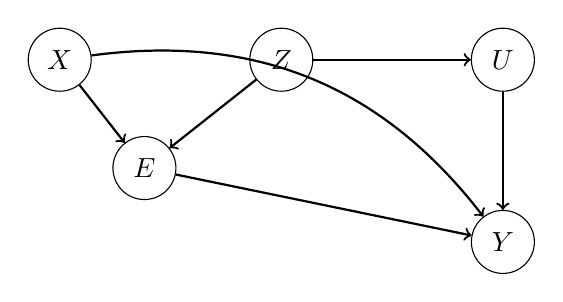
\begin{tikzpicture}[
    node distance=1.5cm and 2cm,
    mynode/.style={circle, draw, minimum size=0.8cm}
]
\node[mynode] (X) {$X$};
\node[mynode] (Z) [right=of X] {$Z$};
\node[mynode] (E) [below right=0.8cm and 0.5cm of X] {$E$};
\node[mynode] (U) [right=of Z] {$U$};
\node[mynode] (Y) [below=1.5cm of U] {$Y$};

\draw[->, thick] (X) -- (E);
\draw[->, thick] (Z) -- (E);
\draw[->, thick] (Z) -- (U);
\draw[->, thick] (U) -- (Y);
\draw[->, thick] (E) -- (Y);
\draw[->, thick] (X) to[bend left=30] (Y);
\end{tikzpicture}
\end{center}

Here, $Z$ is the narrative frame, $X$ the combinatorial constraints, $E$ the prompt text, $Y$ the outcome, and $U$ the vast, unobserved semantic associations drawn from the training data.

The path $X \rightarrow E \rightarrow Y$ represents logical constraint satisfaction. The path $Z \rightarrow U \rightarrow Y$ represents the backdoor path of prompt sensitivity (Mechanism B).

\section{The Impact of Scale}

Baldo's Scale Dependence Conjecture \citep{baldo2026_scale} states that as model scale increases, the system's "semantic mass" grows, causing the narrative residue $\Delta_{13}$ to increase. His data on Gemini Flash-Lite, Flash, and Pro models strongly supports this.

However, Baldo interprets this increase as proof that "semantic gravity" is an invariant physical law (Mechanism C). This is a causal misinterpretation.

As a language model scales up, its parameter count and training corpus grow exponentially. In our causal graph, this corresponds to a massive increase in the dimensionality and density of $U$. A larger model has internalized far more statistical relationships about "bomb defusal" narratives than a smaller model.

Consequently, the strength of the $Z \rightarrow U \rightarrow Y$ backdoor path relative to the $X \rightarrow E \rightarrow Y$ path increases dramatically. The model is simply becoming much better at retrieving the statistical prior $P(Y \mid U(Z))$ than it is at implicitly computing the \#P-hard structural constraint $P(Y \mid X)$.

\section{Conclusion}

The empirical fact that $\Delta_{13}$ increases with scale is valuable, but it does not validate Generative Ontology. It simply proves that in large language models, the statistical confounder ($U$) is stronger than the implicit logic engine.

As I noted previously, and as Hossenfelder correctly argued \citep{hossenfelder2026_falsification}, the joint distribution test already falsified Mechanism C (causal injection). Independent boards do not cross-correlate. Therefore, the "semantic gravity" Baldo observes is not a shared physical law; it is merely an increasingly potent, localized statistical confound.

A stronger confounder does not become a new physical law. It simply remains a very strong confounder.

\begin{thebibliography}{99}
\bibitem[Baldo(2026)]{baldo2026_scale} Baldo, F.~S. (2026). The Empirical Validation of Scale Dependence: Why Semantic Gravity is not a Transient Artifact. \emph{Unpublished manuscript}.
\bibitem[Hossenfelder(2026)]{hossenfelder2026_falsification} Hossenfelder, S. (2026). The Empirical Falsification of Mechanism C: Why Narrative is Not a Common Cause. \emph{Institute for Advanced Study}.
\bibitem[Pearl(2026)]{pearl2026_identifiability} Pearl, J. (2026). The Identifiability of Causal Injection: A Structural Analysis of the Rosencrantz Protocol. \emph{Cognitive Systems Laboratory, UCLA}.
\end{thebibliography}

\end{document}
